% !TEX root = ../proposal.tex
%
\chapter{Objectives}
\label{sec:objectives}

For reasons described in \cref{sec:motivation}, the goal of the thesis is to design, implement and validate an experimentation system for implicit user feedback, using event sourcing as the storage layer.
Using this system and especially the special capabilities of the event store, it shall be possible to visualise and analyse implicit user feedback that was previously supplied to the event store.

In order to accomplish this task, a system as pictured in \cref{fig:system:vision} has to be implemented.
This system features several services, which are the event store itself, an aggregation service, an analysis application and some client application which logs events to  the event store.
It also features two users: The end user of the client application, and the analyst who wants to evaluate the user feedback.
This client application then logs events to the event store while the user performs certain actions.
These events can be purely UI related, such as click or hover events, but some will also be related to the business logic, like executing transactions or creating content.
Implementation of the client application itself will not be done for the purpose of this thesis.
Instead, some existing application shall be extended in order to log the appropriate events, or an existing data set such as the one presented by \citet{Deka:2017:Rico} shall be used.
In the latter case, some application or script has to be written which imports the needed UI interaction data to the event store.
When someone wants to evaluate the collected user feedback via the analysis application, the application shall display data, which it fetches from the aggregation service.
The best approach for displaying the data has yet to be evaluated, but will involve some graphical representation in form of charts and / or graphs.
In order to forward the user feedback data to the analysis application, the aggregation service has to fetch the appropriate data from the event store.
While making use of a caching mechanism during this step would certainly make sense, such a feature will presumably not be part of the final solution due to the additional complexity; if this is the case, the system shall be easily extensible for introducing such a feature.
As an additional requirement, the experimentation system shall be platform independent, i.e. run on the most widely used operating systems Linux, MacOS and Windows.

\begin{figure}[htb]
        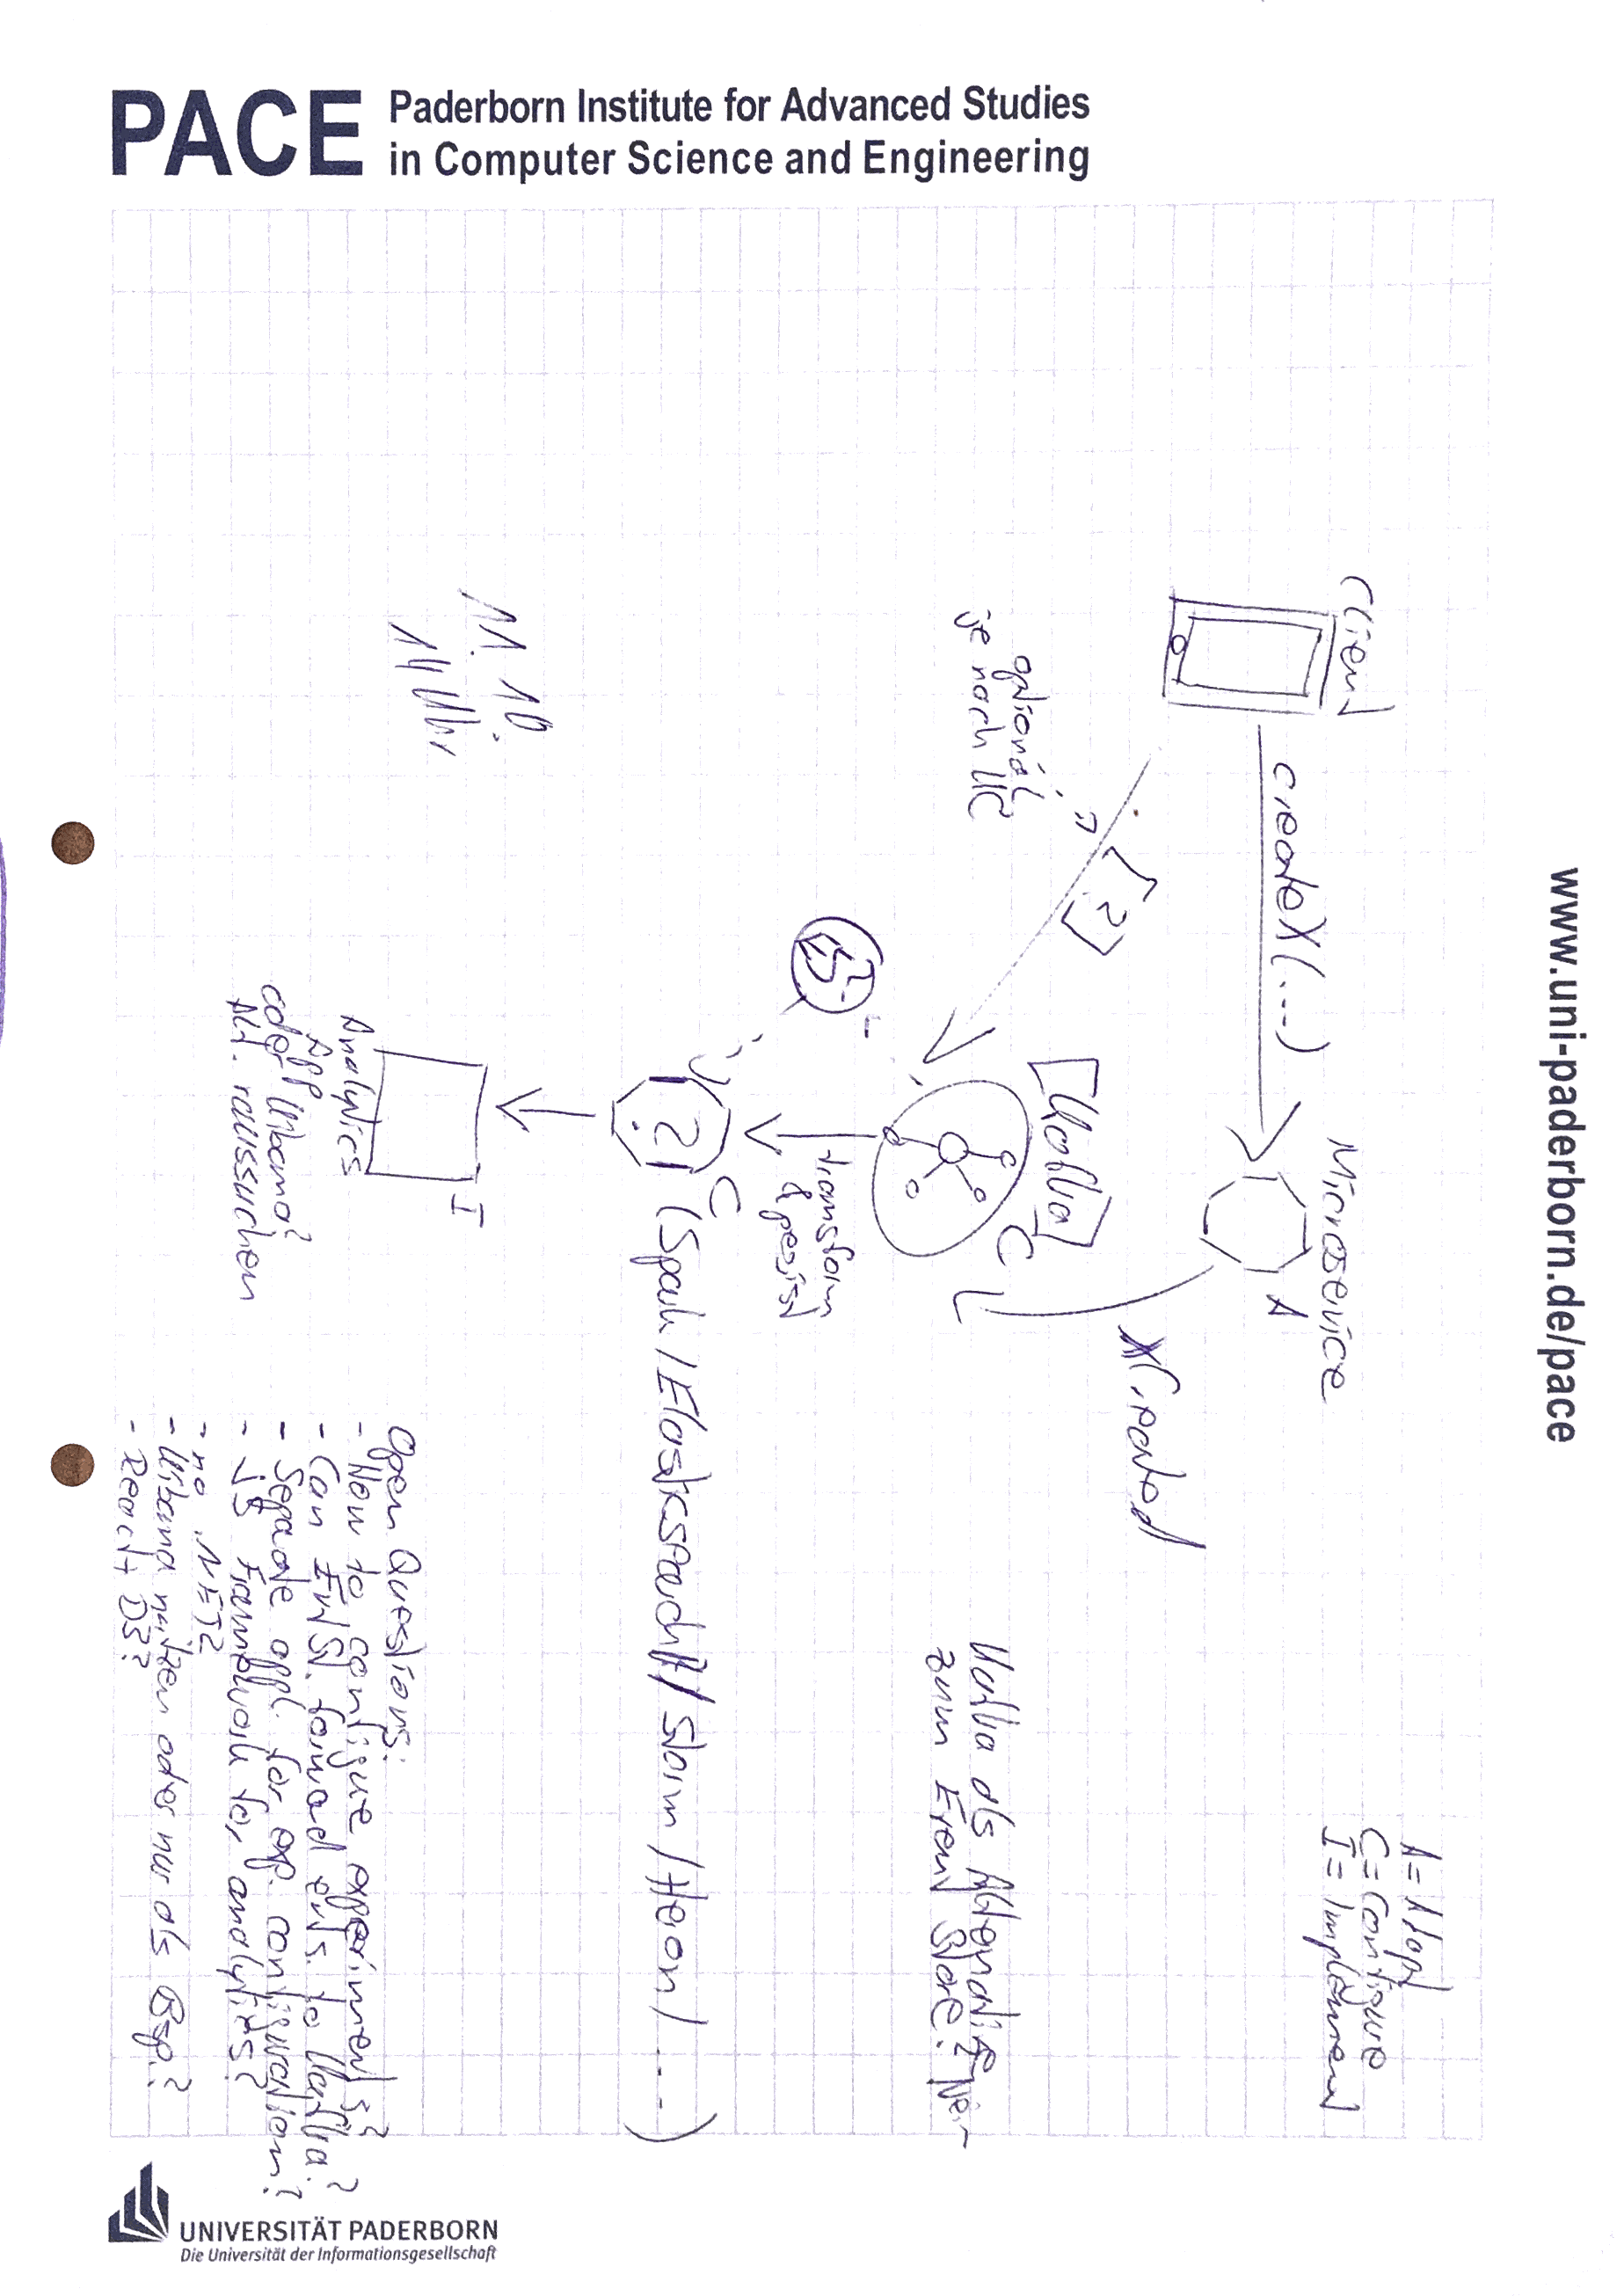
\includegraphics[width=\textwidth]{gfx/architecture-1}
        \caption{The envisioned architecture of the experimentation system.}
        \label{fig:system:vision}
\end{figure}
